\chapter{Koncept}

W niniejszym rozdziale zostanie przedstawiony koncept głównych funkcjonalności projektowanego systemu. Podczas pracy koncepcyjnej autor pracy miał na względzie główny cel systemu jakim jest zrzeszanie zawodników. Proponowane funkcjonalności mają umożliwić osiągnięcie tego celu. Tworząc koncept autor kierował się znajomością potrzeb grupy docelowej, której sam jest częścią, a niejednokrotnie swoje pomysły weryfikował z innymi zawodnikami.
  
  
\section{Baza wiedzy}

W celu umożliwienia zrzeszania zawodników sportów zespołowych konieczne jest przechowywanie w systemie bazy wiedzy na temat zawodników, drużyn oraz obiektów sportowych. W poniższych sekcjach zostaną przybliżone główne założenia dotyczące przechowywania poszczególnych danych.
  
\subsection{Baza zawodników}

Zawodnicy uprawiający amatorsko pewną dyscyplinę sportu są podstawową grupą docelową projektowanego systemu oraz elementem budującym społeczność. Podstawową funkcjonalnością systemu musi być rejestracja zawodników. Podczas procesu rejestracji od użytkownika powinny zostać pobrane dane niezbędne do funkcjonowania systemu, jak również informacje potrzebne do realizacji dalszych założeń, co będzie opisane w kolejnych podpunktach.

\subsection{Baza drużyn}

Zawodnicy po utworzeniu profilu będą mogli założyć drużynę lub dołączyć do już istniejącej drużyny poprzez otrzymanie oraz akceptację zaproszenia. Zawodnik zakładający drużynę otrzymuje specjalną rolę - kapitana. Kapitanem drużyny powinna być osoba reprezentatywna oraz posiadająca dobry kontakt z pozostałymi członkami zespołu, ponieważ to kapitan będzie zajmował się poszukiwaniem przeciwników oraz umawianiem spotkań. Warto zaznaczyć, że kapitan drużyny dalej pozostaje zawodnikiem i może brać czynny udział w rozgrywkach. 

\subsubsection{Punkt macierzysty}

Drużyna powinna wybrać lokalizację, która na potrzeby tej pracy oraz systemu nazwana została "punktem macierzystym". Punkt ten w obrębie systemu będzie służył jako punkt referencyjny dla porównywania odległości pomiędzy drużynami, jak również do oceny odległości od obiektów sportowych. Punktem macierzystym może być na przykład ulubione boisko zawodników lub częste miejsce spotkań pobliskie zawodnikom. W przypadku trudności wyboru domyślną lokalizacją jest centrum regionu, w którym została utworzona drużyna.

\subsection{Baza obiektów sportowych}

Mając na uwadze docelową grupę docelową projektowanego systemu jaką są zawodnicy grający amatorsko - system powinien dostarczać bazę obiektów ogólnodostępnych, a przede wszystkim nie wymagających wkładu finansowego. Głównym konceptem w tym zakresie jest umożliwienie zawodnikom zgłaszania oraz weryfikacji obiektów. 

\section{Wspomaganie poszukiwania rywali}

Kluczową funkcjonalnością systemu jest wspomaganie poszukiwania rywali do gry. Projektując tę funkcjonalność autor pracy miał na względzie, że najważniejszym ogniwem w systemie jest korzystający z niego człowiek. Z tego względu system nigdy będzie podejmował decyzji o wyborze przeciwnika samodzielnie. Celem systemu będzie wspieranie tego procesu poprzez dostarczanie kapitanowi propozycji przeciwników na podstawie zdefiniowanych przez niego preferencji.


\subsection{Kryteria dopasowania}

Podstawowym kryterium dopasowywania drużyn będzie maksymalizacja satysfakcji z gry. Poziom satysfakcji stanowi jednak kryterium, które jest wręcz niemożliwe do ustalenia wprost. Z tego powodu zostały zdefiniowane przesłanki, które mogą wpływać na większą satysfakcję drużyn z rozgrywki:

\begin{itemize}
\item{przybliżony wiek zawodników,}
\item{przybliżony poziom umiejętności zawodników,}
\item{przybliżona forma zawodników,}
\item{zachowanie fair-play drużyny przeciwnej,}
\item{dobre wspomnienia po poprzednich rozgrywkach.}
\end{itemize}

Istotne z punktu widzenia kapitana szukającego przeciwników mogą być również czynniki wpływające na możliwość umówienia spotkania. Mogą być to na przykład informacje dotyczące aktywności drużyny przeciwnej, czy na przykład jej preferowane godziny gry.

Powyższe kryteria będą uwzględnione w projektowanym mechanizmie wspomaganego wyszukiwania przeciwników. Mechanizm powinien zostać zaimplementowany w sposób rozszerzalny, aby możliwe było definiowanie nowych kryteriów wraz z potrzebami rozwojowymi systemu.

\subsection{Problem optymalizacji wielokryterialnej}

Problem optymalizacji wielokryterialnej jest rozszerzeniem problemu optymalizacji jednokryternialnej, gdzie poszukiwana jest decyzja optymalna, ze zbioru możliwych decyzji na podstawie jednego kryterium. Problem ten sprowadza się do poszukiwania maksimum (bądź minimum) funkcji oceny danego kryterium. Jeżeli kryterium jest ilość, np. maksymalna prędkość samochodu, to podejmując decyzje o zakupie jedynie ze względu na to kryterium naturalnie wybierzemy samochód, który osiąga największą prędkość. 

Często jednak podjecie decyzji może być uwarunkowane większą liczbą czynników, na przykład, w przypadku samochodu może to być jego cena, koszt utrzymania, czy czynniki nie ilościowe takie jak jego kolor (w zależności od preferencji kupca). Podejmując decyzje należy rozpatrzyć wiele kryteriów oraz relacje miedzy nimi. Decyzja, która jest optymalna ze względu na jedno z kryteriów, nie musi być optymalna ze względu na pozostałe - z reguły tak nie jest.

\begin{figure}[ht]
\centering
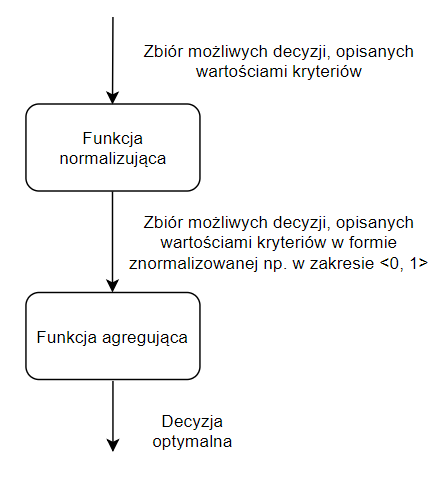
\includegraphics[width=0.5\linewidth]{03-koncept/rys/tradycyjne-algorytmy-opt.PNG}
\caption{Ogólny schemat metody rozwiązywania problemu optymalizacji wielokryterialnej}
\label{fig:diagram-trad-alg-opt}
\end{figure}

Problem podobnej natury występuje w projektowanym systemie. Poszukiwanie rywali do gry można sprowadzić do poszukiwania najlepszych decyzji wyboru drużyny spośród kwalifikujących się drużyn zdefiniowanych w systemie. Przykładowe kryteria wpływające na wartość funkcji oceny dla poszczególnych decyzji (rywali) zostały zdefiniowane w poprzednim podrozdziale.


\subsection{Metoda ważonych kryteriów}

\section{Wspomaganie umawiania się na rozgrywkę}

